Having to take care of managing multiple trucks, truck drivers, their turns, their parking lots
and their parking spaces can be a difficult task to achieve, especially when you have to deal with
time management, availability, delays, and so on.
However, going by old systems, either an Excel spreadsheet or just a ledger system on
paper, can help such a task, as long as you're working on a small scale. But once
this scales, the need for assistance grows.

And that's the point where comes the possibility to make use of automated tasks to do the job.
Automating the management, making it easier to manage with as little human intervention
as possible.

As of the current time, there is already a solution put in place, which is a SaaS hosted
on AWS implementing an SOA architecture. The SaaS relies on various managed services
provided by AWS, such as EC2, S3, RDS, etc.

The MMSoft Saas is constituted of:
\begin{itemize}
    \item Four front-end services:
    \begin{itemize}
        \item Easy-truck-in (ETI) interface which is the main interface
        \item Driver application (Angular 11)
        \item Registration Tablet App (React 16)
        \item Gatekeeper App (Cermate)
    \end{itemize}
    \item Four Back-end services:
    \begin{itemize}
        \item MQTT Broker communicating with the Gatekeeper app (VerneMQ)
        \item Orchestration Back-end Service (Java 11 Spring Boot 2.6) used by the ETI interface
        \item Registration Service (Node JS 16) used by the Registration Tablet App
        \item TMS Registration Back-end which exposes REST API for integration (Java 11 Spring Boot 2.6)
    \end{itemize}
    \item Two databases:
    \begin{itemize}
        \item MySQL for users, site, configuration
        \item Redis as a database for Daily/Weekly data and for messaging communication with other services
    \end{itemize}
\end{itemize}


And it has the following backend service used, as shown in the figure below:

\begin{center}
    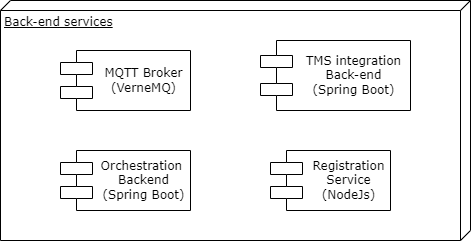
\includegraphics[width=0.8\textwidth]{images/Backend}
\end{center}



